%&latex
%
\providecommand{\main}{../..}
\documentclass[../../main.tex]{subfiles}

\begin{document}

\section{Proof that $\mathbb{P}(m,t) \to \mathbb{P}_{\mathrm{eq.}}(m)$}\label{sec:proof-db}\lesson{30}{18/05/20}

\textbf{Hypotheses}. 
Assume that:
\begin{enumerate}
    \item \textbf{Detailed balance} (\ref{eqn:detailed-balance}) holds:
    \begin{align}\label{eqn:hyp-db1}
        {W(m|m') \mathbb{P}_{\mathrm{eq}}(m')} = {W(m'|m) \mathbb{P}_{\mathrm{eq}}(m)} 
    \end{align}
    \item For any pairs of states $(m,m')$, there is a \textbf{path} $\{m_0 = m, m_1, m_2, \dots, m_K = m'\}$ with \textbf{non-zero transition rate}:
    \begin{align}\label{eqn:hyp-2}
        W(m_K|m_{K-1}) W(m_{K-1}|m_{K-2}) \cdots W(m_1|m_0) > 0
    \end{align}
    In other words, there is a way to go from every state $m$ to any other state $m'$ in a finite number of steps. 
\end{enumerate}
\begin{figure}[H]
    \centering
    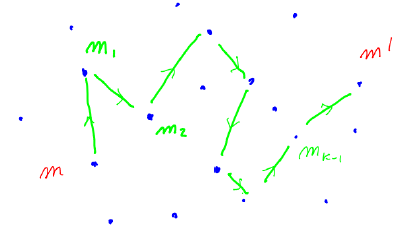
\includegraphics[width=0.8\textwidth]{\main/path_existance.png}
    \caption{Any pair of states of $(m,m')$ must have a \textit{possible} path that connects them.}
    \label{fig:path_existance}
\end{figure}
\textbf{Thesis}. 
Then, we want to show that:
\begin{align*}
    \lim_{t \to +\infty} \mathbb{P}(m,t) = \mathbb{P}_{\mathrm{eq}}(m)
\end{align*}
Moreover, we are interested in finding a way to compute \textit{how fast} $\mathbb{P}(m,t)$ goes to $\mathbb{P}_{\mathrm{eq}}$.

\medskip

\textbf{Sketch of proof}. 
The idea of the proof is to solve the evolution differential equation in matrix form (\ref{eqn:pdf-evolution-matrixform}):
\begin{align}\label{eqn:evo-matrixform}
    \dot{\bm{P}}(t) = \mathrm{T} \bm{P}(t) \qquad \mathrm{T}(m,m') \equiv W(m|m') - \delta_{m,m'} \sum_{m''} W(m''|m')
\end{align}
This is a system of first order differential equations. To solve it, we make use of the \textbf{spectral decomposition} of $\mathrm{T}$.

Let $\{\bm{w_n}\}$ be a orthonormal basis\marginpar{Idea of the proof} of $\mathbb{R}^N$, with $\bm{w_n}$ being the eigenvectors of $\mathrm{T}$ with eigenvalues $\lambda_n \in \mathbb{R}$:
\begin{align}\label{eqn:eigen-eq}
    \mathrm{T} \bm{w_n} = \lambda_n \bm{w_n} \qquad \langle \bm{w_n}, \bm{w_m} \rangle = \delta_{n,m}
\end{align}

Then we can write any vector $\bm{P} \in \mathbb{R}^N$ as a linear combination of $\{\bm{w_n}\}$:
\begin{align}\label{eqn:Pt}
    \bm{P}(t) = c_1(t) \bm{w_1} + \dots + c_N(t) \bm{w_N} = \sum_{n} c_n(t) \bm{w_n}
\end{align}

Differentiating:
\begin{align*}
    \dot{\bm{P}}(t) = \sum_n \dot{c}_n(t) \bm{w_n} \underset{(\ref{eqn:evo-matrixform})}{=}  \mathrm{T} \sum_{n} c_n(t) \bm{w_n} \underset{(\ref{eqn:eigen-eq})}{=} \sum_n \lambda_n c_n(t) \bm{w_n} 
\end{align*}
If we then take the scalar product of both sides with $\bm{w_m}$ and apply the orthonormality property (\ref{eqn:eigen-eq}) we get:
\begin{align*}
    \dot{c}_m(t) = \lambda_m c_m(t) \qquad \forall m = 1,\dots,N
\end{align*}
which can immediately be solved by separation of variables:
\begin{align*}
    c_m(t) = c_m(0) e^{\lambda_m t}
\end{align*}
And substituting back in (\ref{eqn:Pt}) we find the solution:
\begin{align*}
    \bm{P}(t) = \sum_n c_n(0) e^{\lambda_n t} \bm{w_n}
\end{align*}

To proceed, we will show that $\mathbb{P}_{\mathrm{eq}}$ is an eigenvector of $\mathrm{T}$ with eigenvalue $\lambda_0 = 0$, and that all other eigenvectors have $\lambda_n < 0$. This means that, for any initial condition:
\begin{align*}
    \bm{P}(t) = \sum_n c_n(0) e^{\lambda_n t} \bm{w_n} = c_0(0) \mathbb{P}_{\mathrm{eq}} + \sum_{n > 0} c_n(0) e^{-|\lambda_n|t} \bm{w_n}  \xrightarrow[t \to \infty]{}  c_0(0) \mathbb{P}_{\mathrm{eq}}
\end{align*}
Due to the conservation of probability $c(0) = 1$. Moreover, if $\lambda_1$ is the eigenvalue nearest to $0$, it describes the \textit{dominant} timescale for reaching $\mathbb{P}_{\mathrm{eq}}$. 

\medskip

So, to complete the proof we will proceed as follows:
\begin{enumerate}
    \item First we show that a orthonormal eigenbasis of $\mathrm{T}$ (\ref{eqn:eigen-eq}) exists, and that the eigenvalues $\lambda_n$ are real. This is done by showing that, by just rescaling $\mathrm{T} \mapsto \hat{T}$ (which does not alter the eigenvalues), it becomes a \textbf{symmetric} matrix.
    \item Then we show explicitly that $\mathbb{P}_{\mathrm{eq}}$ is the eigenvector with $0$ eigenvalue, and that all the other $\lambda_n$ are negative. 
    \item We will adapt the previous arguments to the newly defined matrix $\hat{T}$.
\end{enumerate}

\textbf{Proof}.

\begin{enumerate}
    \item To \q{symmetrize} $\mathrm{T}$, we first \textit{symmetrize} $W$, starting by dividing both sides of (\ref{eqn:hyp-db1}) by $\sqrt{\mathbb{P}_{\mathrm{eq}}(m) \mathbb{P}_{\mathrm{eq}}(m')}$ (assuming $\mathbb{P}_{\mathrm{eq}}(m) \neq 0$ $\forall m$):
    \begin{align}\label{eqn:symmetric-db}
        W(m|m') \sqrt{\frac{\mathbb{P}_{\mathrm{eq}}(m')}{\mathbb{P}_{\mathrm{eq}}(m)}} = W(m'|m) \sqrt{\frac{\mathbb{P}_{\mathrm{eq}}(m)}{\mathbb{P}_{\mathrm{eq}}(m')} }
    \end{align}
    For simplicity of notation, let's define:
    \begin{align}\label{eqn:What}
        \hat{W}(m|m') \equiv W(m|m') \sqrt{\frac{\mathbb{P}_{\mathrm{eq}}(m')}{\mathbb{P}_{\mathrm{eq}}(m)} }
    \end{align}
    Then (\ref{eqn:symmetric-db}) can be written as:
    \begin{align*}
        \hat{W}(m|m') = \hat{W}(m'|m)
    \end{align*}
    meaning that the matrix $\hat{W}_{m,m'} \equiv \hat{W}(m|m')$ is symmetric.
    
    \medskip
    
    We apply the same transformation (\ref{eqn:What}) to the matrix $T$ defined in (\ref{eqn:T-matrix}):
    \begin{align} \label{eqn:That}
        \hat{T}(m,m') &\equiv T(m,m') \sqrt{\frac{\mathbb{P}_{\mathrm{eq}}(m')}{\mathbb{P}_{\mathrm{eq}}(m)}} =\\
        \nonumber
        &= \underbrace{W(m|m') \sqrt{\frac{\mathbb{P}_{\mathrm{eq}}(m')}{\mathbb{P}_{\mathrm{eq}}(m)}}}_{\hat{W}(m,m')} - \delta_{m,m'} \sum_{m''} \sqrt{\frac{\mathbb{P}_{\mathrm{eq}}(m')}{\mathbb{P}_{\mathrm{eq}}(m)}} W(m''|m') = \\ \nonumber
        &\underset{\mathclap{(a)}}{=} \hat{W}(m,m') - \delta_{m,m'} \sum_{m''} \sqrt{\frac{\mathbb{P}_{\mathrm{eq}}(\textcolor{Red}{m})}{\mathbb{P}_{\mathrm{eq}}(m)} } W(m''|m') =\\ \nonumber
        &= \hlc{Yellow}{\hat{W}(m,m') }- \hlc{SkyBlue}{\delta_{m,m'} \sum_{m''} W(m''|m')}
    \end{align}
    where in (a) we note that the second term can be non-zero only if $m = m'$ (due to the $\delta$) and in this case the two $\mathbb{P}_{\mathrm{eq}}$ factors cancel out.
    
    The matrix $\hat{T}$ is the sum of a symmetric matrix $\hat{W}$ (yellow term) and a diagonal matrix (blue term), so it is symmetric:
    \begin{align*}
        \hat{\mathrm{T}}(m,m') = \hat{\mathrm{T}}(m',m)
    \end{align*}
    Since $\hat{\mathrm{T}}$ is symmetric, its eigenvectors $\{\bm{v_n}\}$ form a basis of $\mathbb{R}^N$, and may be chosen to be orthonormal:
    \begin{align*}
        \hat{\mathrm{T}} \bm{v_n} = \lambda_n \bm{v_n} \qquad \langle \bm{v_n}, \bm{v_m} \rangle = \delta_{n,m}
    \end{align*}

    Moreover, the eigenvalues of $\hat{\mathrm{T}}$ are \textbf{real} numbers (since $\hat{\mathrm{T}}$ has real entries), and are the same of the eigenvalues of $\mathrm{T}$, since the trasnformation $\mathrm{T} \mapsto \hat{\mathrm{T}}$ is a \textbf{similitude} transformation, i.e. (\ref{eqn:That}) may be written as:
    \begin{align*}
        \hat{\mathrm{T}} = S^{-1} \mathrm{T} S \qquad S_{m,m'} = \delta_{m,m'} \sqrt{\mathbb{P}_{\mathrm{eq}}(m)}
    \end{align*} 
    
    The eigenvectors of $\mathrm{T}$ and $\hat{\mathrm{T}}$, on the other hand, are different. In fact, if $\bm{v_n}$ is an eigenvector of $\hat{\mathrm{T}}$ with eigenvalue $\lambda_n$ then:
    \begin{align}\nonumber
        \hat{\mathrm{T}} \bm{v_n} &= \lambda_n \bm{v}_n \\ \nonumber
        \Rightarrow  S^{-1} \mathrm{T} S \bm{v}_n &= \lambda_n \bm{v}_n\\ \nonumber
        \Rightarrow  \mathrm{T} \underbrace{S \bm{v}_n}_{\bm{w_n^R}}  &= \lambda_n \underbrace{S \bm{v}_n}_{\bm{w_n^R}} \\
        \Rightarrow  \mathrm{T} \bm{w_n^R} &= \lambda_n \bm{w_n^R}
        \label{eqn:right-eigenvector}
    \end{align}
    where $\bm{w_n^R} = S \bm{v_n}$ is the right eigenvector of $\mathrm{T}$ corresponding to the eigenvector $\bm{v_n}$ of $\hat{\mathrm{T}}$.

    \medskip

    Transposing the eigenvalue equation we obtain also an expression for the left eigenvectors of $\mathrm{T}$:
    \begin{align}\nonumber
        \bm{v_n}^T \hat{\mathrm{T}} &= \lambda_n \bm{v_n}^T\\
        \Rightarrow  \bm{v_n}^T S^{-1} \mathrm{T} S &=  \lambda_n \bm{v_n}^T\\ \nonumber
        \Rightarrow \bm{v_n}^T S^{-1} \mathrm{T} &= \lambda_n \bm{v_n}^T S^{-1}\\ \nonumber
        \Rightarrow [(S^{-1})^T \bm{v_n}]^T \mathrm{T} &= \lambda_n [\underbrace{(S^{-1})^T \bm{v_n}}_{\bm{w_n^L}}]^T \\
        \Rightarrow [\bm{w_n^L}]^T \mathrm{T} &= \lambda_n [\bm{w_n^L}]^T 
        \label{eqn:left-eigenvector}
    \end{align}
    \item We know that $\mathbb{P}_{\mathrm{eq}}$ is a stationary state, and so $\dot{\mathbb{P}}_{\mathrm{eq}} = 0$. Substituting this in (\ref{eqn:pdf-evolution-matrixform}) we get:
    \begin{align}\label{eqn:Peq-stationarity}
        \mathrm{T} \mathbb{P}_{\mathrm{eq}} = 0
    \end{align}
    And so $\bm{w_0^R} = \mathbb{P}_{\mathrm{eq}}$ is a right eigenvector of $\mathrm{T}$. This means that:
    \begin{align*}
        \bm{v_0} \underset{(\ref{eqn:right-eigenvector})}{=}  S^{-1} \mathbb{P}_{\mathrm{eq}} = (1/\sqrt{\mathbb{P}_{\mathrm{eq}}^{(k)}} \colon k = 1,\dots,N)^T
    \end{align*}
     is a right eigenvector of $\hat{\mathrm{T}}$, with eigenvalue $0$.

    \medskip

    We now prove that all the other $\lambda_n$ are negative. Starting from the eigenvalue equation for $\hat{\mathrm{T}}$ and taking the scalar product of both sides by $\bm{v_n}$ we get:
    \begin{align*}
        \langle \bm{v_n}, \hat{\mathrm{T}} \bm{v_n} \rangle = \lambda \underbrace{\langle \bm{v_n}, \bm{v_n} \rangle}_{1} 
    \end{align*}
    So $\lambda_n < 0$ ($n > 0$) if and only if $\langle \bm{v}, \hat{\mathrm{T}}\bm{v} \rangle < 0$ $\forall \bm{v} \in \mathbb{R}^N \setminus \{\bm{0}\}$. Let's write this scalar product in full:
    \begin{align}\nonumber
        \langle \bm{v}, \hat{\mathrm{T}} \bm{v} \rangle &= \sum_{m,n} v_m \hat{\mathrm{T}}_{mn} v_n \underset{(\ref{eqn:That})}{=} \sum_{mn} v_m v_n \sqrt{\frac{\mathbb{P}_{\mathrm{eq}}(n)}{\mathbb{P}_{\mathrm{eq}}(m)}} \left[W(m|n) - \delta_{mn} \sum_k W(k|m) \right] =\\ \nonumber
        &= \sum_{mn} v_m v_n \sqrt{\frac{\mathbb{P}_{\mathrm{eq}}(n)}{\mathbb{P}_{\mathrm{eq}}(m)}} W(m|n) - \sum_{kn} v_n^2 W(k|n)
        \intertext{In the last term we used the $\delta_{mn}$ to remove the sum over $m$ by setting $m = n$. Then, if we rename $k \leftrightarrow m$ we can merge the two sums:}
        &= \sum_{mn} \left[v_m v_n \sqrt{\frac{\mathbb{P}_{\mathrm{eq}}(n)}{\mathbb{P}_{\mathrm{eq}}(m)}} W(m|n)- v_n^2 W(m|n)\right] \label{eqn:sum-merge}
    \end{align}
    Since the sum is over both $m$ and $n$, note that:
    \begin{align*}
        \sum_{mn} v_{\textcolor{Red}{n}}^2 W(\textcolor{Blue}{m}|\textcolor{Red}{n}) = \sum_{mn} v_{\textcolor{Blue}{m}}^2 W(\textcolor{Red}{n}|\textcolor{Blue}{m})
    \end{align*}
    This allows to \textit{symmetrize} the last term in (\ref{eqn:sum-merge}):
    \begin{align}\label{eqn:symm-term}
        \sum_{mn} v_n^2 W(m|n) = \frac{1}{2} \left[\sum_{mn} v_n^2 W(m|n) + \sum_{mn} v_m^2 W(n|m)\right]  
    \end{align}
    In this way we can use (\ref{eqn:hyp-db1}) to express $W(n|m)$ in terms of $W(m|n)$ and $\mathbb{P}_{\mathrm{eq}}$:
    \begin{align}\label{eqn:db-cons}
        W(n|m) = W(m|n) \frac{\mathbb{P}_{\mathrm{eq}}(n)}{\mathbb{P}_{\mathrm{eq}}(m)} 
    \end{align}

    Substituting (\ref{eqn:symm-term}) and (\ref{eqn:db-cons}) in (\ref{eqn:sum-merge}) we can finally recognize a square:
    \begin{align}\nonumber
        \langle \bm{v}, \hat{\mathrm{T}} \bm{v} \rangle &= \frac{1}{2} \sum_{mn} W(m|n) \mathbb{P}_{\mathrm{eq}}(n) \left[2 \frac{v_m}{\sqrt{\mathbb{P}_{\mathrm{eq}}(m)}} \frac{v_n}{\sqrt{\mathbb{P}_{\mathrm{eq}}}(n)} - \left(\frac{v_n}{\sqrt{\mathbb{P}_{\mathrm{eq}}(n)}} \right)^2 - \left(\frac{v_m}{\sqrt{\mathbb{P}_{\mathrm{eq}}(m)}} \right)^2  \right] =\\
        &= -\frac{1}{2} \sum_{mn} W(m|n) \mathbb{P}_{\mathrm{eq}}(n) \left(\frac{v_n}{\sqrt{\mathbb{P}_{\mathrm{eq}}(n)}} - \frac{v_m}{\sqrt{\mathbb{P}_{\mathrm{eq} }(m)}}  \right)^2 \leq 0 \label{eqn:square}
    \end{align}

    In particular the equality is reached if:
    \begin{align}\label{eqn:equality-pair}
        \frac{v_n}{\sqrt{\mathbb{P}_{\mathrm{eq}}(n)}} = \frac{v_m}{\sqrt{\mathbb{P}_{\mathrm{eq}}(m)}}  \qquad \forall n,m \colon W(m|n) > 0
    \end{align}
    However, by hypothesis there is \textit{always} a path connecting any pair of states $(m,n)$, meaning that $W(m|n) > 0$ always. So (\ref{eqn:equality-pair}) must hold for every pair $(m,n)$, which is only possible if it's constant:
    \begin{align*}
        \frac{v_n}{\sqrt{\mathbb{P}_{\mathrm{eq}}(n)}} = \text{Constant independent of $n$} \equiv c
    \end{align*}
    So $\bm{v_0} \in \mathbb{R}^N$ with entries given by:
    \begin{align*}
        v_n = c \sqrt{\mathbb{P}_{\mathrm{eq}}(n)}
    \end{align*}
    is the \textbf{only} eigenvector of $\hat{\mathrm{T}}$ with eigenvalue $0$. If we choose $c=1$, the corresponding eigenvector of $T$ is exactly $\mathbb{P}_{\mathrm{eq}}$:
    \begin{align*}
        \sum_n \hat{\mathrm{T}}(m,n)\sqrt{\mathbb{P}_{\mathrm{eq}}(n)} &= \sum_n T(m,n) \sqrt{\frac{\mathbb{P}_{\mathrm{eq}}(n)}{\mathbb{P}_{\mathrm{eq}}(m)} } \sqrt{\mathbb{P}_{\mathrm{eq}}(n)} =\\
        &= \frac{1}{\sqrt{\mathbb{P}_{\mathrm{eq}}(m)}} \sum_n T(m,n) \mathbb{P}_{\mathrm{eq}}(n) \underset{(\ref{eqn:Peq-stationarity})}{=}  0
    \end{align*}
    Then, all the other eigenvalues $\lambda_n$ ($n > 1$) are negative.
    \item Finally, let's wrap up the demonstration. Since $\hat{\mathrm{T}}$ is symmetric, we can choose an orthonormal basis $\{\bm{v_n}\}$ made by eigenvectors of $\hat{\mathrm{T}}$. Let's denote with $\{\bm{w}_n^L\}$ and $\{\bm{w_n^R}\}$ the corresponding left and right eigenvectors of $\mathrm{T}$. Each of the two sets still form a (non-orthonormal) basis of $\mathbb{R}^N$.
    
    We have:
    \begin{align}\label{eqn:on-2}
        \delta_{n,m} = \langle \bm{v_n}, \bm{v_m} \rangle = \langle \bm{w_n^L} S, S^{-1} \bm{w_n^R} \rangle = \langle \bm{w_n^L}, \bm{w_n^R} \rangle
    \end{align}

    We can write $\bm{P}(t)$ as a linear combination of $\{\bm{w_n^R}\}$:
    \begin{align}\label{eqn:Pt2}
        \bm{P}(t) = \sum_{k} c_k(t) \bm{w_k^R} \qquad c_k(t) = \langle \bm{w_k^L}, \bm{P}(t) \rangle
    \end{align}
    Differentiating:
    \begin{align*}
        \partial_t \bm{P}(t) &= \sum_{k} \dot{c}_k(t) \bm{w_k^R} = \mathrm{T} \bm{P}(t) = \sum_k c_k(t) \mathrm{T} \bm{w_k^R}= \sum_k c_k(t) \lambda_k \bm{w_k^R}
    \end{align*}
    And taking the scalar product of both sides with $\bm{w_j^L}$ and applying (\ref{eqn:on-2}) leads to:
    \begin{align*}
        \dot{c}_j(t) = \lambda_j c_j(t) \Rightarrow c_j(t) = c_j(0) e^{\lambda_j t}
    \end{align*}
    Substituting back in (\ref{eqn:Pt2}):
    \begin{align*}
        \bm{P}(t) = \sum_{k} c_k(0) e^{\lambda_k t} \bm{w_k^R}  \xrightarrow[t \to +\infty]{} c_0(0) \underbrace{\bm{w_0^R}}_{\mathbb{P}_{\mathrm{eq}}} 
    \end{align*}
    In particular:
    \begin{align*}
        c_0(0) = \langle \bm{w_0^L}, \bm{P}(t=0) \rangle
    \end{align*}
    And $\bm{w_0^L} = (1,\dots,1)^T$ because:
    \begin{align*}
        (1,\dots,1)^T \mathrm{T} &= \sum_{m} \mathrm{T}_{mn} \underset{(\ref{eqn:T-matrix})}{=}  \sum_m W(m|n) - \sum_m \delta_{mn} \sum_{k} W(k|n) =\\
        &= \sum_{m} W(m|n) - \sum_k W(k|n) \>\> \underset{\mathclap{k \leftrightarrow m}}{=} \>\> \sum_m \cancel{W(m|n)} - \sum_m \cancel{W(m|n)} = 0
    \end{align*}
    Thus, as $\bm{P}$ is a vector of probabilities that must sum to $1$:
    \begin{align*}
        c_0(0) = \langle \bm{1}, \bm{P}(t=0) \rangle = \sum_n P_n(0) \overset{!}{=} 1
    \end{align*}

    This proves indeed that:
    \begin{align*}
        \bm{P}(t)  \xrightarrow[t \to +\infty]{}  \mathbb{P}_{\mathrm{eq}}
    \end{align*}
\end{enumerate}

\textbf{Alternative proof}. The same result can be deduced on the basis of the time behaviour of the relative entropy (\ref{eqn:relative-entropy}). Recall that the relative entropy can be regarded as measuring a sort of \q{distance} between different probabilities distributions. In particular, if we compar $\bm{P}(t)$ with the equilibrium distribution $\mathbb{P}_{\mathrm{eq}}$, the relative entropy is given by:
\begin{align*}
    S_R(t) \equiv - \sum_m \mathbb{P}(m,t) \ln \frac{\mathbb{P}(m,t)}{\mathbb{P}_{\mathrm{eq}}(m)} 
\end{align*} 
Recall that $S_R(t) \leq 0$, with the equality reached only if $\mathbb{P}(m,t) = \mathbb{P}_{\mathrm{eq}}(m)$ $\forall m$.

\medskip

Differentiating both sides:
\begin{align*}
    \partial_t S_R(t) &= -\sum_m \left[\dot{\mathbb{P}}(m,t) \ln \frac{\mathbb{P}(m,t)}{\mathbb{P}_{\mathrm{eq}}(m)} + \mathbb{P}(m,t) \frac{\dot{\mathbb{P}}(m,t)}{\mathbb{P}(m,t)} \right] =\\
    &\underset{(\ref{eqn:MasterEquation})}{=}  -\sum_{mn} \left[W(m|n) \mathbb{P}(n,t) - W(n|m)\mathbb{P}(m,t)\right] \ln \frac{\mathbb{P}(m,t)}{\mathbb{P}_{\mathrm{eq}}(m)} - \underbrace{\sum_m \cancel{\dot{\mathbb{P}}(m,t)}}_{\mathclap{0 \> (\text{Prob. conserv.})}} 
\end{align*}
In the first term, as we are summing over both $m$ and $n$, we can use again the trick of summing the same expression with $m \leftrightarrow n$ and then dividing by $2$:
\begin{align*}
    \partial_t S_R(t) &= -\frac{1}{2} \sum_{mn} \left[W(m|n)\mathbb{P}(n,t) - W(n|m) \mathbb{P}(m,t)\right] \left[\ln \frac{\mathbb{P}(m,t)}{\mathbb{P}_{\mathrm{eq}}(m)} - \ln \frac{\mathbb{P}(n,t)}{\mathbb{P}_{\mathrm{eq}}(n)}  \right]
\end{align*}
We can rewrite the logarithms as follows:
\begin{align*}
    \ln \frac{\mathbb{P}(m,t)}{\mathbb{P}_{\mathrm{eq}}(m)} - \ln \frac{\mathbb{P}(m,t)}{\mathbb{P}_{\mathrm{eq}}(m)} = \ln \left[\frac{\mathbb{P}(m,t)}{\mathbb{P}(n,t)} \frac{\mathbb{P}_{\mathrm{eq}}(n)}{\mathbb{P}_{\mathrm{eq}}(m)} \right]
\end{align*}
and then use the detailed balance condition:
\begin{align*}
    \frac{\mathbb{P}_{\mathrm{eq}}(n)}{\mathbb{P}_{\mathrm{eq}}(m)}  = \frac{W(n|m)}{W(m|n)} 
\end{align*}
so that:
\begin{align*}
    \partial_t S_R(t) &= \frac{1}{2} \sum_{mn} \left[\underbrace{W(m|n)\mathbb{P}(n,t)}_{x} -\underbrace{ W(n|m) \mathbb{P}(m,t)}_{y}\right] \ln \frac{W(m|n)\mathbb{P}(n,t)}{W(n|m)\mathbb{P}(m,t)} =\\
    &= \frac{1}{2} (x-y) \ln \frac{x}{y} = y \left(\frac{x}{y} -1 \right) \ln \underbrace{\frac{x}{y}}_{z} = y(z-1) \ln z
\end{align*}
Note that $y > 0$ and $z > 0$ (as they are a product/ratio of positive quantities). So $(z-1)\ln z \geq 0$, with the equality reached only if $z=1$. Thus:
\begin{align*}
    \partial_t S_R(t) \geq 0
\end{align*}
In particular:
\begin{align*}
    \partial_t S_R(t) = 0 \Leftrightarrow \frac{W(m|n)\mathbb{P}(n,t)}{W(n|m)\mathbb{P}(m,t)} = 1 \Leftrightarrow \mathbb{P}(m,t) = \mathbb{P}_{\mathrm{eq}}(m) \frac{\mathbb{P}(n,t)}{\mathbb{P}_{\mathrm{eq} }(n)}  \quad \forall m,n
\end{align*}
since we have assumed that all pairs of states are joined by a path of non-zero transition rates $W(i|j)$.

\medskip

Summing over $m$:
\begin{align*}
    \sum_m \mathbb{P}(m,t) = 1 = \frac{\mathbb{P}(n,t)}{\mathbb{P}_{\mathrm{eq}}(n)} \underbrace{\sum_m \mathbb{P}_{\mathrm{eq}}(m) }_{1} \Rightarrow \frac{\mathbb{P}(n,t)}{\mathbb{P}_{\mathrm{eq}}(n)} = 1  
\end{align*}
Thus:
\begin{align*}
    \partial_t S_R(t) = 0 \Leftrightarrow \mathbb{P}(m,t) = \mathbb{P}_{\mathrm{eq}}(m)
\end{align*}

Summarizing, we know that $S_R(t)$ is bounded ($S_R(t) \leq 0$), and for every initial condition different from the equilibrium ($\mathbb{P}(m,0) \neq \mathbb{P}_{\mathrm{eq}}(m)$) it increases with time ($\partial_t S_R(t) > 0$). Since $S_R(t)$ is monotonous and bounded, it admits a limit for $t \to +\infty$, that we denote with $S_R^*$:
\begin{align*}
    \lim_{t \to +\infty} S_R(t) \equiv S_R^*
\end{align*}
This limit \textit{must} be $S_R^* = 0$, meaning that $\mathbb{P}(m,t)  \xrightarrow[t \to \infty]{}  \mathbb{P}_{\mathrm{eq}}(m)$. In fact, if we assume by absurd that $\mathbb{P}(m,t)  \xrightarrow[t \to \infty]{}   \mathbb{P}^*(m) \neq \mathbb{P}_{\mathrm{eq}}(m)$, then $S_R^* < 0$ and the time derivative would be positive in the limit:
\begin{align*}
    \partial_t S_R(t)  \xrightarrow[t \to \infty]{}  \frac{1}{2} \sum_{mn} [W(m|n) \mathbb{P}^*(n) - W(n|m)\mathbb{P}^*(m)] \ln \frac{W(m|n)\mathbb{P}^*(n)}{W(n|m)\mathbb{P}^*(m)} > 0
\end{align*}
which is absurd, since $S_R(t)$ is bounded, and so it cannot increase indefinitely. So, this proves that:
\begin{align*}
    \lim_{t \to +\infty} \mathbb{P}(m,t) = \mathbb{P}_{\mathrm{eq}}(m) \quad \forall m
\end{align*}
However, differently from the previous proof, we do not have any information on the \textit{rate} of convergence (which we know to be exponential).

\chapter{Population Dynamics}
Population dynamics is the branch of life sciences that studies the \textbf{size} and \textbf{composition} of populations as \textbf{dynamical systems}. In particular, it aims to model the growth and disappearence of species in ecosystems, allowing to understand the impact of changes in the environment on \textbf{biodiversity} - a topic of utmost importance in the current times, more than ever.

\medskip

In this chapter, \textit{population dynamics} will serve us as a \q{test range} to appreciate the \textbf{power} and \textbf{generality} of statistical mechanics. 

\medskip

After a brief introduction, we will focus on several historical models, and see how the techniques we developed in the previous chapters (e.g. variational principle, mean field approximation, scaling laws) can be effectively used to solve problems. As we will show, often just trying to simplify complex systems in terms of paradigmatic models of statistical mechanics, such as the Ising Model, can reveal deep similarities between very different subjects - developing insight on important physical phenomena.

\section{Historical notes}
At its most basic, population dynamics models how the number of individuals of a given species changes with time.

One of the first attempt to describe\marginpar{Fibonacci sequence} a population was made by Fibonacci back in the 13th century, resulting in the popular \textbf{Fibonacci sequence}.

The main focus was to describe the unchecked growth of a \textit{idealized} colony of \textit{rabbits}, with the following assumptions:
\begin{itemize}
    \item Each pair of adult rabbits mates after one month, generating a new pair.
    \item Newly born rabbits grow to adulthood in just one month.
    \item The environment resources are abundant, and so rabbits may breed forever
\end{itemize}
If we start with a single pair of rabbits ($N_0=1$), the total population $N$ will grow as follows:
\begin{enumerate}
    \item In the first month, the only pair of rabbits just grows to adulthood, without generating a new pair, so $N_1=1$.
    \item In the second month, the pair of adult rabbits will produce a new pair, leading to $N_2=2$.
    \item In the third month, the original pair of rabbits will produce a new pair, but the second pair needs still some time to grow. So we have $N_3 = 3$.
    \item In the fourth month, two pairs of rabbits reproduce, and so $N_4 = 5$
\end{enumerate}
It can be shown that:
\begin{align*}
    N_n = N_{n-1} + N_{n-2}
\end{align*}
with $N_0 = 0$ and $N_1 = 1$. This is the recurrence relation of the so-called \textbf{Fibonacci sequence}, which is now so famous to have gained an exclusive mathematical journal\footnote{\url{https://www.fq.math.ca/}}.

\medskip

The Fibonacci sequence\marginpar{Euler} is one of the first description of \textit{exponential growth}. A more detailed account on the same concept was given several years later by \textbf{Euler} in a treaty about the infinite \cite{euler_population}.

\medskip

One of the most influential works\marginpar{Malthus} on population dynamics was the \q{Essay on the Principle of Population} written by \textbf{Malthus} in 1798. Its main observation was that human population increased \textit{geometrically}, while resources only \textit{linearly} (Malthusian Law of Population). Without any active control on birth rates, this would have lead to overpopulation and famine. 

Malthus book motivated the \textit{Census Act} in the 1800 Britain, starting a detailed account of all population every $10$ years. 

\medskip

All of these models, however,\marginpar{Verhulst} focused heavily on describing the exponential \textit{growth} of population. It was Verhulst, in 1838, to consider quantitatively the environmental \textbf{limiting effects}. He modelled the population $p(t)$ with a differential equation as follows:
\begin{align*}
    \dv{p}{t} = mp - \phi(p)
\end{align*}
Here $m$ is is a constant describing \textit{fertility}, i.e. the rate of growth of population, while $\phi(p)$ is a (non-linear) unknown function acting as a \textit{limiter}. In this way, population grows exponentially only at the start, and then \textit{stabilizes} at a certain point, due to mortality and lack of resources - both of which scale on $p$ (more population means, for instance, a higher probability for epidemics and famine). This is the first example of a \textit{logistic growth}.

\medskip

The \textbf{interaction} between different\marginpar{Lotka-Volterra} species was initially examined in a landmark work of the 1920s, where the dynamics of two populations - predator and prey - was described by two coupled differential equations by Lotka and Volterra:
\begin{align*}
    \begin{cases}
        \dv{N_1}{t} = (\epsilon_1 - \gamma_1(h_1 N_1 + h_2 N_2))N_1\\
        \dv{N_2}{t} = (\epsilon_2 - \gamma_2(h_1 N_1 + h_2 N_2))N_2
    \end{cases}
\end{align*}
Both populations tend to increase exponentially with a rate $\epsilon_{1,2}$, but they are limited by a Verhulst non-linear term ($N_{1,2}^2$) and also by the size of the other population. %Check constants
The result is that $N_1(t)$ and $N_2(t)$ both \textit{oscillate} with the same period, but with a slight offset in their phase. If the prey increases, than predators will have more food and increase, reducing the number of prey, meaning that now predators will find more difficult to find nourishment, and so on. A behaviour of this kind was effectively observed in nature, by studying the population of fish.

\medskip

While Lotka-Volterra approach involved \textbf{deterministic} differential equations, the same behaviour can be modelled using \textbf{stochastic processes}, and in particular the so-called \textbf{birth-death processes}. The main results are the same, but the stochastic case exhibits some interesting consequences due to its inherent \textit{randomness}, such ast the phenomenon of \textit{stochastic amplification}, where significant oscillations in the population are produced by fluctuations and amplified by interaction. We will dedicate one of the following sections to introducing some simple birth-death processes.

\medskip

In \textbf{modern times}, population dynamics is fueled by an increasingly available \textbf{ecological data}. For example there are 5-year census of entire tree populations in the Amazon, registering many features of interest.

\medskip

One of the first to try to understand biodiversity and biogeography in a mathematical way is \textbf{Stephen Hubbel}, who wrote \q{The Unified Neutral Theory of Biodiversity and Biogeography} in 2001. He proposed that the complexity of biodiversity could be unsterstood with very \textbf{simple models}, and tried to simplify complex models of the past so that they can be more maneageable.

\section{Features of interest}
In the rest of the chapter, we will present several \textit{models} of population dynamics, finding interesting application to statistical mechanics techniques. Before doing that, however, let's examine \textit{what exactly} are we trying to describe.   

\medskip

The main focus of population dynamics has always been the \textit{counting} of individuals belonging to a population (e.g. a certain \textit{species}). 

The distribution of species\marginpar{$\alpha$-diversity} sizes in an ecosystem, i.e. the probability that a given species picked at random has exactly $n$ individuals, is called the $\bm{\alpha}$-\textbf{diversity} of that ecosystem. It is inherently a measure of \textit{biodiversity}, giving us some information abouth the \textit{health} of a certain population - for example trees in an Amazon rainforest.

We know that the existence of many different species is important to maintain a sort of \q{stable equilibrium} in nature, i.e. ecosystems with less \textit{variety} are more prone to extinction, and more sensitive to external perturbations. This is particularly relevant when studying the distribution of bacteria species in the human gut, since here changes can lead to disease.  

\medskip

$\alpha$-diversity can be studied as a function of \textit{time}, i.e. in the evolution of ecosystems; or \textit{space}, i.e. how it scales with area. In the latter case, it is unsurprising to find that the number of individuals usually \textit{scales linearly} with the considered area, as if any species had a fixed spatial \textbf{density} (fig. \ref{fig:constant-density}).

\begin{figure}[H]
    \centering
    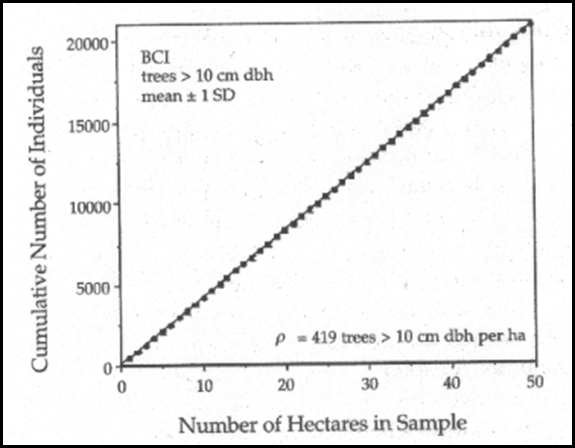
\includegraphics[width=0.7\textwidth]{\main/Images/constant-density.png}
    \caption{Population size of trees in the Barro Colorado Island (BCI) forest as a function of the sample area.}
    \label{fig:constant-density}
\end{figure}

In terms of frequency, $\alpha$-diversity gives us information about the \textbf{Relative Species Abundance} (RSA), i.e. how many individuals of a given species are present in a certain sample of population.

\medskip

To measure the \textbf{interaction} between different\marginpar{$\beta$-diversity} species, we can consider the \textbf{two-point correlation function}, i.e. the probability of finding a certain species $i$ at a fixed distance $r$ from a species $j$. This is the so-called $\bm{\beta}$-diversity. It is also an example of inherently \textbf{spatial feature}. 
%another question: why biodiversity depends heavily on latitude? It is nearly constant near the equator, but drops fast at higher latitudes. 
\medskip

$\alpha$, $\beta$-diversity and other spatial features can be determined by available empirical data. The challenge is then to find a \textit{understandable} model that, given some \q{simple assumptions}, is able to \textit{fit} that data and \textit{predict} how it evolves in time. In particular, we already know that real systems exhibit \textit{scaling laws} similar to those of physical systems at criticality - so we will pay additional attention to finding them.


\section{Neutral theory}
At first, the problem of studying many different species, each one with unique \textit{quirks} and \textit{interactions}, can seem intractable with relatively simple models. It is reasonable that the complex biodiversity of an Amazon rainforest would require hundreds of parameters to be tackled - which would quickly destroy any hope of some real understanding.

\medskip

Fortunately, this is not the case. Complex ecosystems are surprisingly \textit{simple} at their core: to the eye of population dynamics, all species \q{look the same}, and almost \textit{do not} interact with each other. This is the main argument of the \textbf{neutral theory} by Stephen Hubbell: all species which share the same \textit{level} in the food chain can be considered \textit{equivalent}, in the sense that differences between them are \q{neutral}, i.e. irrelevant to the success of their individuals. 

\medskip

From a physical point of view, this is great news: it means that we can create models with \textit{few} parameters, borrowing ideas from the paradigmatic models of statistical mechanics, and achieve our target. Still, the extraordinary nature of such a claim requires a strong foundation.

\medskip

In this introduction, we will consider just an example at the root of the neutral theory. Let's consider an Amazon rainforest, inhabited by many different species of trees. If the assumptions of neutral theory are adequate, we expect all trees to be placed \q{at random}, i.e. without any correlation to other physical quantities. 

Let's consider, for example, the distribution of \textbf{nutrients} in an area (fig. \ref{fig:relative-nutrients}). This is done by dividing the area in small \textit{quadrants}, and measuring in each of them the relative concentration of certain soil elements.

\begin{figure}[H]
    \centering
    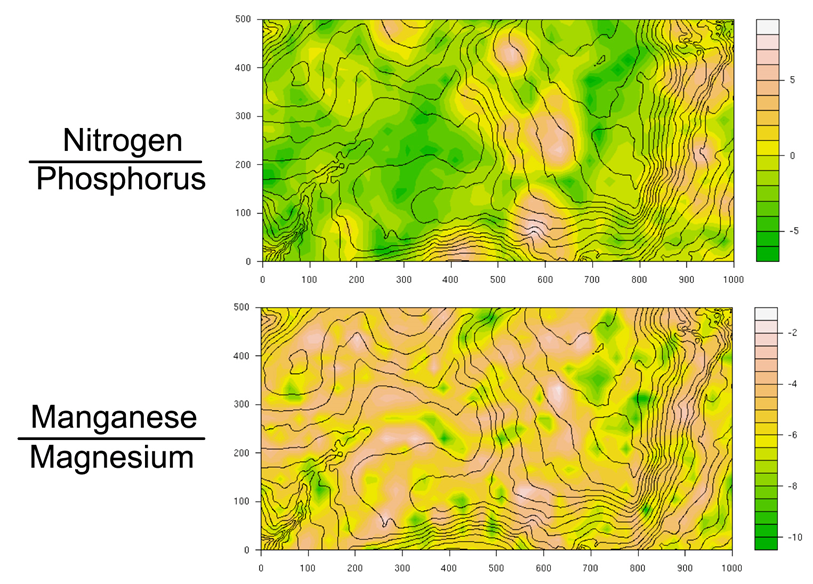
\includegraphics[width=0.8\textwidth]{\main/Images/relative-nutrients.png}
    \caption{Relative distribution of plant nutrients in the BCI forest}
    \label{fig:relative-nutrients}
\end{figure}

We then consider all the quadrants with a given concentration of nutrients, and measure in them the \textit{relative abundance} of tree species, i.e. the fraction of all individuals in these quadrants that belong to a given species. For example, suppose that a species $A$ is \textit{specialized} in consuming phosphorus, and a species $C$ instead prefers \textit{nitrogen}. Then we would expect to find a lot of trees of species $A$ in quadrants where the ratio nitrogen/phosphorus is low, and a lot of trees of species $C$ where it is high, giving rise to a plot similar to fig. \ref{fig:N-P-plot}.

\begin{figure}[H]
    \centering
    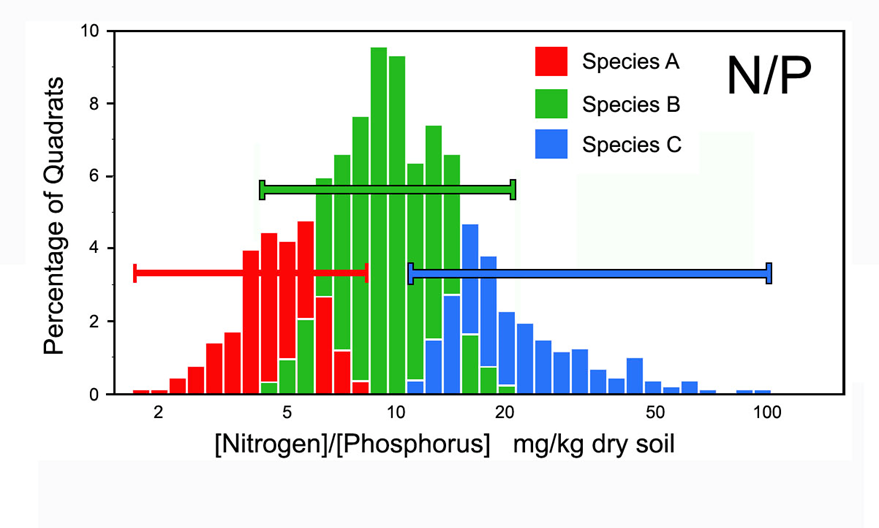
\includegraphics[width=0.8\textwidth]{\main/Images/N-P-plot.png}
    \caption{Relative abundance of nutrient-specialized species}
    \label{fig:N-P-plot}
\end{figure}

However, when plotting \textit{real data}, we do not see this kind of pattern. Instead, species seem to be \textit{agnostic} to the relative concentration of nutrients - they simply occupy all available space (fig. \ref{fig:hybanthus}).

\begin{figure}[H]
    \centering
    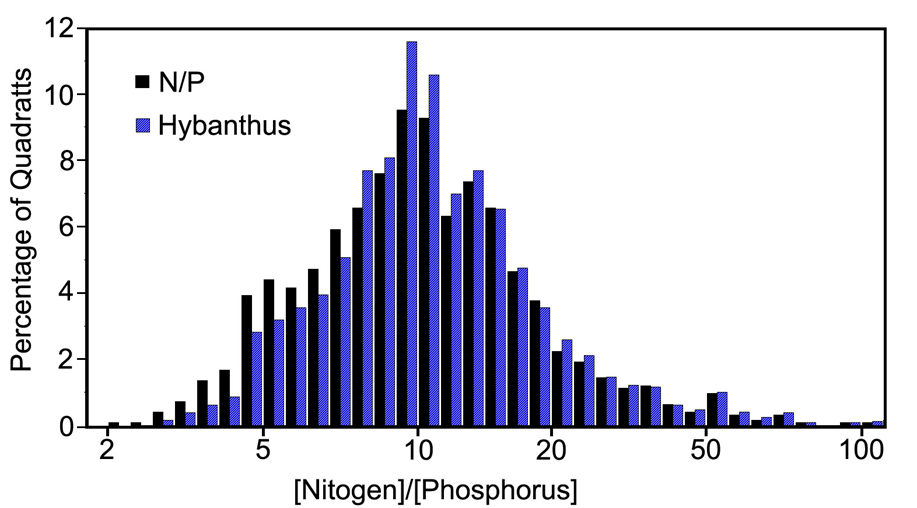
\includegraphics[width=\textwidth]{\main/Images/hybanthus.png}
    \caption{The distribution of hybanthus as a function of soil nutrients concentration. There is no clear \textit{bias} towards a certain element.}
    \label{fig:hybanthus}
\end{figure}

The same result holds for different combinations of nutrients and different species, contributing evidence for the neutral assumption.

\medskip
\end{document}
